\chapter{Introduction}

%Libraries are quite useful to make standard knowledge available to users, so they can just focus on the novelty of their task. Libraries of Mathematics are no exception. 
%Building a large library of mathematics is one of the goals of the mechanized mathematics and formal knowledge communities. It has been envisioned by the QED manifesto in 1994 \ednote{cite}, and has - since then - been the subject of many research efforts \ednote{citations}. 

%Formalizing a mathematical result is a lot of work, involving a lot of subtleties and design decisions. 

A software system is more useful to its users when it is equipped with a library of ready-to-utilize information. A user can then focus on what is novel and more interesting to them. When it comes to Mathematics, the amount of information that can be contained in such a library is huge. The influential QED manifesto~\cite{boyer1994qed}, released in 1994, envisioned a library in which all Mathematics is formalized and rigorously checked. The QED manifesto believed in one-formalization-fits-all approach to building the library. 
As the mathematics knowledge management community grew larger, the vision for the large math library has been reframed into a collection of heterogeneous, intercommunicating systems, under the name universal digital math library (UDML)~\cite{farmer2004mkm}. Despite all the efforts to build such a library, it still does not exist. We focus our attention on algebra libraries. They mostly contain three types of definitions 
\begin{itemize}
    \item Theories describing algebraic structures, like \lstmath{Monoid}, \lstmath{Group}, and \lstmath{Ring}. 
    \item Constructions related to these algebraic structures, like morphisms, products, and term algebras.  
    \item Proofs of basic theorems. 
\end{itemize}

Current practice involves having library developers write all definitions by hand. We want to support the activity of library building by providing more automation to this process. We build our system based on $2$ observations. We discuss them here using the theory of \lstmath{Monoid} as our running example.  

% QED has been revised in .. , attributing its non realization to not enough man power (due to the lack of an immediate application) and that formalized mathematics is not good for communication, and does not resemble classic mathematics.  \ednote{say more here}.

%There were many problems with the realization of this library, \ednote{citations}, of which we focus on two; capturing the structure of Mathematics and the huge manpower needed to formalize this information. We focus our attention to libraries of Algebra. 

\paragraph{Variabilities in theory presentations}
%A UDML will contain a huge amount of mathematical knowledge Beside the shear volume of information that needs to be included in a large math library, there is a large variability in design decisions within the systems and between the projects using them. Even for one piece of mathematical information, there are different ways of presenting it. We will focus on libraries of Algebra and use \lstmath{Monoid} as our running example. 
The theory of \lstmath{Monoid} in Mathematics describes an algebraic structure that has a carrier, a binary operation which is associative and has a unit. 
Figure~\ref{fig:mon-diff-lang} shows how the \lstmath{Monoid} theory is defined in $5$ different languages. Those definitions are mathematically equivalent, but they look different because they are expressed in different logics and based on different design decisions. 
\begin{figure}
    \footnotesize
\begin{tabular}{p{6.3cm} p{7cm}}
\underline{Haskell}
\begin{minted}[mathescape]{haskell}
class Semigroup a => 
      Monoid a 
 where 
  mempty :: a 
  mappend :: a -> a -> a 
  mappend = (<>) 
  mconcat :: [a] -> a 
  mconcat = 
   foldr mappend mempty 
\end{minted} 
\underline{Lean}
\begin{leancode}
class monoid (M : Type u)
 extends semigroup M, 
         has_one M :=
  (one_mul : ~$\forall$~ a : M, 
           1 * a = a) 
  (mul_one : ~$\forall$~ a : M, 
           a * 1 = a)   
\end{leancode} 
% [mathescape=true, escape_inside=~~]
\underline{Coq}
\begin{minted}[mathescape=true, escapeinside=~~]{coq}
class Monoid {A : type}
 (dot : A ~$\to$~ A ~$\to$~ A)
 (one : A) : Prop := {
  dot_assoc : 
   forall x y z : A, 
   (dot x (dot y z)) = 
   dot (dot x y) z
  unit_left : forall x, 
   dot one x = x 
  unit_right : forall x, 
   dot x one = x              
}
~$\text{\textit{Alternative Definition:}}$~
Record monoid := {
 dom : Type; 
 op : dom -> dom -> dom 
  where "x * y" := op x y; 
 id : dom where "1" := id; 
 assoc : forall x y z, 
  x * (y * z) = (x * y) * z; 
 left_neutral : forall x,   
  1 * x = x; 
 right_neutal : forall x,
  x * 1 = x; 
}
\end{minted} 
&
\underline{Agda}
\begin{agdacode}
record Monoid c ~$\ell$~ : 
   Set (suc (c ~$\sqcup$~ ~$\ell$~)) where 
 infixl 7 _~$\bullet$~_
 infix 4 _~$\approx$~_
 field 
  Carrier : Set c 
  _~$\approx$~_ : Rel Carrier ~$\ell$~ 
  _~$\bullet$~_ : Op~$_2$~ Carrier 
  isMonoid : IsMonoid _~$\approx$~_ _~$\bullet$~_ ~$\varepsilon$~ 
  
record IsMonid (~$\bullet$~ : Op~$_2$~) (~$\varepsilon$~ : A) 
 : Set (a ~$\sqcup$~ ~$\ell$~) where 
  field 
   isSemiring : IsSemiring ~$\bullet$~ 
   identity : Identity ~$\varepsilon$~ 
       
   open IsSemigroup isSemigroup public 
   
   identity~$^l$~ : LeftIdentity ~$\varepsilon$~ ~$\bullet$~ 
   identity~$^l$~ = proj~$_1$~ identity 
   identity~$^r$~ : Rightdentity ~$\varepsilon$~ ~$\bullet$~ 
   identity~$^r$~ = proj~$_2$~ identity        
\end{agdacode}       
\underline{MMT}
\begin{minted}[mathescape=true, escapeinside=~~]{mmt} 
theory Semigroup : ?NatDed = 
 u : sort 
 comp : tm u ~$\to$~ tm u ~$\to$~ tm u 
  # 1 * 2 prec 40
 assoc : ~$\vdash$~ ~$\forall$~ [x, y, z]
  (x * y) * z = x * (y * z)    
 assocLeftToRight : 
  {x,y,z} ~$\vdash$~ (x * y) * z 
          = x * (y * z) 
  = [x,y,z] 
   allE (allE (allE assoc x) y) z
 assocRightToLeft : 
  {x,y,z} ~$\vdash$~  x * (y * z) 
           = (x * y) * z 
  = [x,y,z] sym assocLR 
theory Monoid : ?NatDed 
 includes ?Semigroup 
 unit : tm u # e 
 unit_axiom : ~$\vdash$~ ~$\forall$~ [x] = x * e = x       
\end{minted}      
\end{tabular}  

    \caption{Representation of \lstinline|Monoid| theory in different languages.}
    \label{fig:mon-diff-lang}
\end{figure}

In some cases, as in Haskell and MMT, the theory \monoid is defined as an extension of \semigroup. Despite this being useful, there is no reason why a developer might not want to add a theory \unital (a non-associative \monoid), to the hierarchy. Exposing this hierarchy to the user makes their code vulnerable in case the hierarchy changes. This problem occurred when Haskell changed the hierarchy of type classes when \lstmath{Applicative} became a superclass for \lstmath{Monad} ~\cite{wiki:haskell_hierarch}. The work in \cite{cohen2020hierarchy} discusses this problem. 
%A better approach to defining \monoid here would consider it to be an extension of both theories, but still allowing the user to overlook the hierarchy and deal with the \emph{flattened} definition, if that all they need to get their work done. \ednote{maybe I want to move this argument from here}. 

The two Coq definitions takes two extreme views to the bundling problem~\cite{lean2019,alhassy2019,spitters2011type} by either having the carrier and all the function symbols as arguments (the first definition) or having all elements of the theory as declarations of a record type (the second definition). 

The formalization of the Algebraic hierarchy in the Agda standard library is based on setoids (sets equipped with the equivalence relation). Therefore, we find an extra field of the definition of \monoid corresponding to the equivalence relation $\_\approx\_$. 

These variabilities reflect the design decisions of library builders and makes it harder to customize these definitions for users' projects that choose different decisions. This usability problem leads to redundancy as users are forced to redefine theories for their own purposes. We find multiple libraries for the algebraic hierarchy, even within the same system. In the Coq system, there are at least $4$ libraries of Algebra~\cite{Gonthier2009,Geuvers2002,coq-contribs-algebra,Spitters2010}, and even more for Category Theory~\cite{spivak2014coqcats}. In 
\cite{Gonthier2009}, the authors
mention, referring to other libraries:  
\begin{quote}
    ``In spite of this body of prior work, however, we have found it
    difficult to make practical use of the algebraic hierarchy in our project to
    formalize the Feit-Thompson Theorem in the Coq system."
\end{quote}

\paragraph{Handwritten Boilerplate}
Libraries provide some utilities related to algebraic structures, including signatures, morphisms, term languages, etc. 
Figure~\ref{fig:hom-foo-bar} shows the definition of homomorphism for two theories within the same language; \lstmath{Foo} and \lstmath{Bar}. 
\begin{figure}
\begin{multicols}{2}
  \begin{lstlisting}[mathescape]
theory Foo { 
  U : type 
  s1 : U 
  s2 : U $\to$ U $\to$ U
}

theory FooHom{
  f1 , f2 : Foo 
  hom : f1.U $\rightarrow$ f2.U 
  pres-s1 : ... 
  pres-s2 : ... 
}
\end{lstlisting}        
\columnbreak
\begin{lstlisting}[mathescape]
theory Bar {
  U : type 
  s1 : U 
  s2 : U $\rightarrow$ U 
}

theory BarHom { 
  b1, b2 : Bar 
  hom : b1.U $\rightarrow$ b2.U 
  pres-s1 : $\cdots$
  pres-s2 : $\cdots$
}
\end{lstlisting}
\end{multicols}    
\caption{Definition of homomorphisms for two theories}
\label{fig:hom-foo-bar}
\end{figure}

To define the homomorphism in both cases, we need to define two instances of the theory, a homomorphism function from the carrier of the first one, to the carrier of the second, and the preservation axioms that follow the pattern
\begin{lstlisting}[mathescape]
hom (op$_1$ x$_1$ .. x$_n$) = op$_2$ (hom x$_1$) .. (hom x$_n$)
\end{lstlisting} 

There are many other constructs that follow from the definitions of theories. We discuss them in Section\ednote{Add this in the future}. The presentation of those constructs change based on the different design decisions employed by the system. In case the carrier is a parameter to the theories \lstmath{Foo} and \lstmath{Bar}, the definition of homomorphism would look different. 

Optimally, our library will have definitions of those constructions for every algebraic structure and would be adaptable to the different design decisions. 

\paragraph{}
Current practice is that library developers take a lot of design decisions upfront to defining the theories, and they become core parts of it. They also provide all definitions of related constructions manually. It takes a huge amount of human work to provide all the definitions within a large library of mathematics; Add to this the requirement that those definitions becomes customizable so they can serve multiple user needs. 

We want to enhance this practice by providing more automation to the process of library development. We suggest a generative approach in which a developer can \emph{describe} what information needs to go in the library and what design decisions they are taking, then the library gets generated based on this description. 

We are inspired by the \emph{deriving} mechanism in Haskell. When defining a new datatype, a Haskell user can ask for some utilities to be readily available for them to use on that type. The Haskell compiler would then generate these functions for the user. Some of these are basic, like equality and printer, but the community has gone as far as giving users the chance to define their own templates for deriving instances, knows as the \emph{deriving-via} technique. A pretty impressive example of deriving information is shown in Figure~\ref{fig:deriving-via-example}\ednote{find a better way to put the link to the source}. 
Also, the Lens library~\cite{lensesLib} in Haskell, use template Haskell~\cite{sheard2002TH} for the same purpose. 
\begin{figure}
 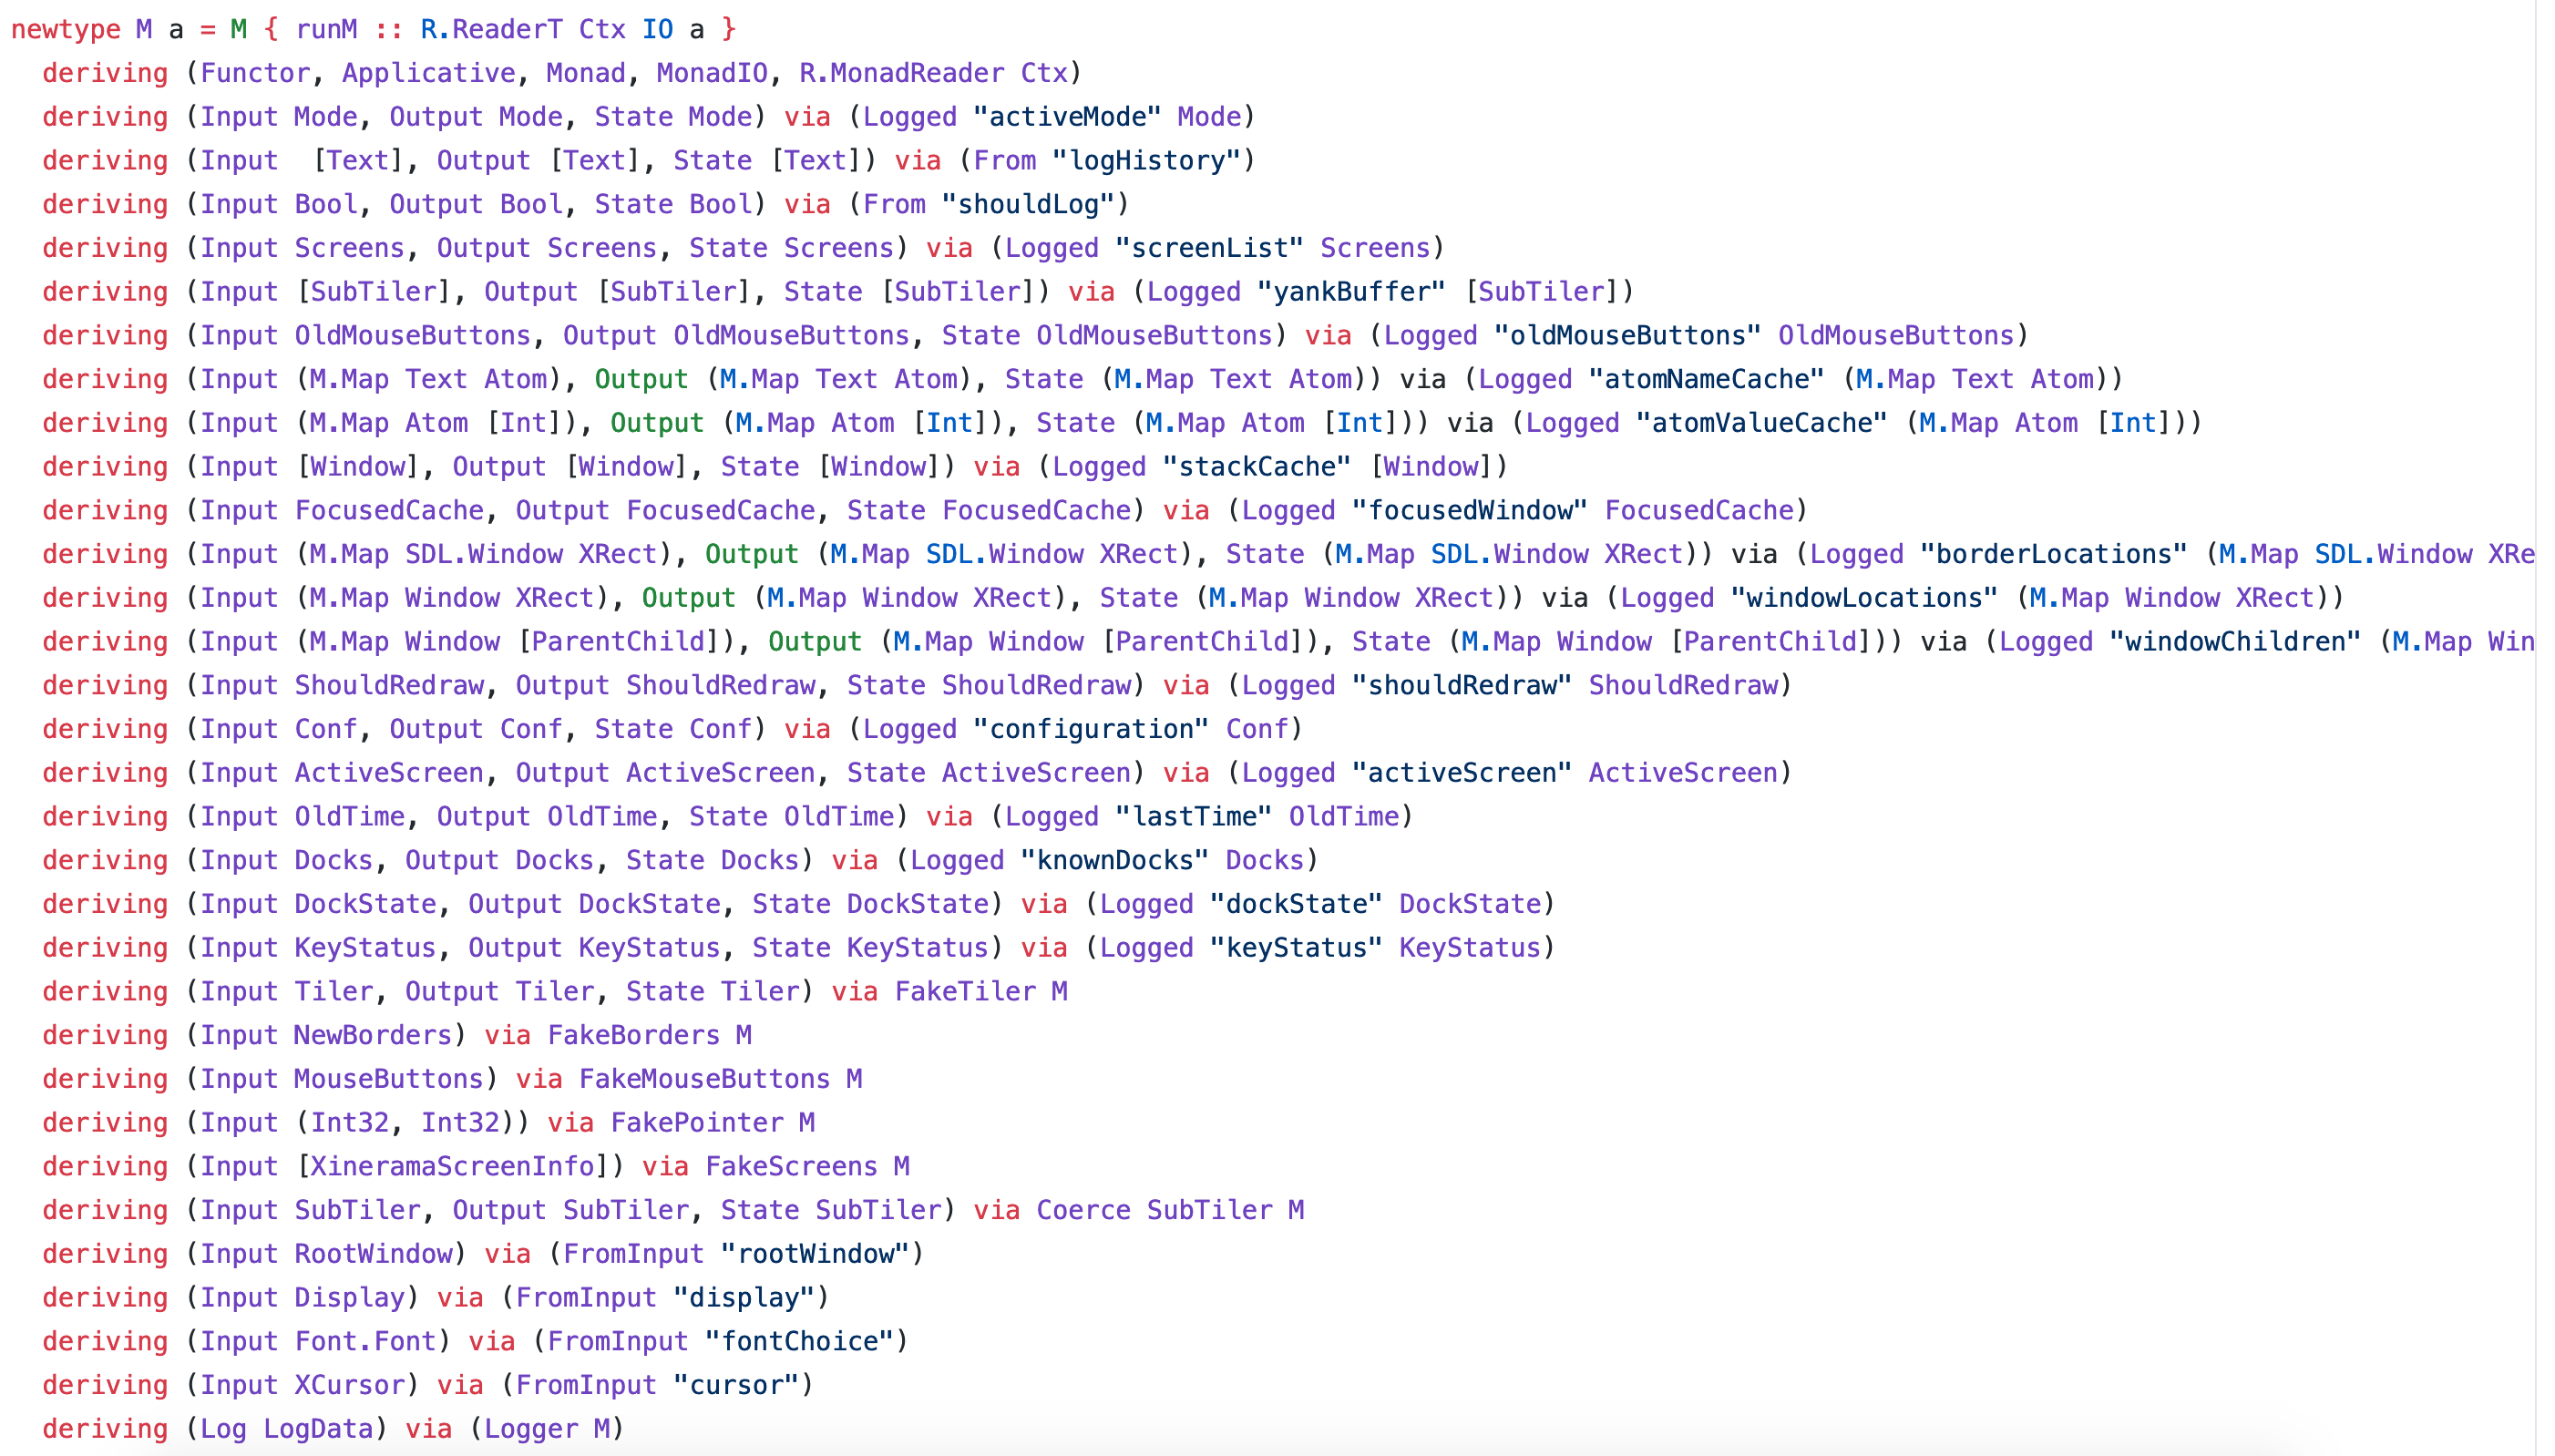
\includegraphics[scale=0.5,width=\linewidth]{figures/deriving-via-example.png}
 \caption{Example of deriving information in Haskell. source:\url{https://github.com/jhgarner/Xest-Window-Manager/blob/3741b35a69eb2cf8cd7320e186fd40134d1c1a56/src/Base/DoAll.hs}}
 \label{fig:deriving-via-example}
\end{figure}

%We are suggesting the use of automation to improve library building and enhance the reusability of its definitions. First, we use an abstraction over details of theory presentations It appears to be inevitable that to improve reusability, we need to have multiple presentations of a theory, and accordingly, multiple presentations of its related constructions. But a library developer should not be writing these definitions by hand. 
%In this work, we suggest  Users can then load the version of \lstmath{Monoid} that works better for their purposes. 

\section{Research Problem}

We work towards providing a DSL for theory development that can be used for building libraries and developing theories within users' projects. It would lift the burden of having to define utilities that are needed to perform the task in hand, but are standard information to the point that writing them is boring and distracting from the original task. 

\paragraph{Why?}
Having this DSL in place would benefit the process of theory development in the following ways 
\begin{itemize}
    \item Reduce the development time of new libraries by providing expressions instead of actual definitions 
    \item Enhance the maintainability of the library. By understanding how new design decisions affect the definitions, developers would modify the generator instead of having to modify every definition. 
    \item Increase the usability of library definitions by giving the users the tools to customize those definitions.  
\end{itemize}  

\paragraph{How?}
In order to develop this DSL we need to find out the right abstraction from which all the variabilities and the related constructions can be generated and we also need to provide an interpreter for this DSL that generates the library definitions. 

Universal algebra provides us with the right abstractions. It abstracts over algebraic structures and their related constructions and provides the meta theory that explains how the generation algorithms should work. A theory presentation in universal algebra has three components \verb|(S,F,E)|; a sort \verb|S|, a list of function symbols along with their arities \verb|F|, and a list of axioms (equations) that describe properties of the function symbols \verb|E|. If we can abstract over the details of theory presentations to extract this information, we are able to generate the constructions defined by universal algebra, like morphisms, product algebras, term languages, $\cdots$, etc. 


Also, we know that theory presentations are written in formal languages, which provide uniform syntax for expressing information. By having a suitable way to manipulate theories, we can generate information from them. This can happen if theories are first class citizens, if the needed reflection mechanisms are in place, or using a meta program in the hosting language. We use Tog~\cite{tog} as our language and type checker. We discuss Tog in Chapter~\ref{ch:tog}. 

%First, it is loaded with design decisions that are not relevant to the mathematical definitions. Second that many of the information provided in the library does not have to be written by hand, but can be automatically generated if enough machinery is in place. 

%Current practice is that library developers make choices with respect to these attributes and stick to it. This creates a reusability problems in projects that do not want to stick with those choices and a maintainability problem in case the library developer changes their decisions. These decisions propagates to constructions that are related to algebraic structures, adding to the overhead of redefining this information. \ednote{The existence of multiple definitions that support variabilities in design decision is desirable redundancy}

%We want to support library builders, by lifting the burden of having to define information that can be automatically computed if given the appropriate description. We want to use generative programming to achieve that, working towards a DSL for library building. In this model, one gives a description of what needs to be in the library, then an interpreter would automatically generate the definitions. This way, we can achieve highly reusable, easily maintainable library, requiring less human effort. 

In this work, we attempt to answer the following research questions 
\begin{itemize}
    \item Can the uniformity provided by universal algebra be captured by a meta program that generates parts of an algebra library?
    \item What design decisions need to be abstracted from? and which ones can be reintroduced after the generation of new?
    \item Which information need to be provided by the developer and which ones can be generated? 
    \item What are the preconditions for generating this new information? 
    \item How would this affect the activity of library building?
    \item Can the generation algorithms be extended beyond the library, to user-defined theories?
    \item Can these generation algorithms be extended beyond uni-sorted first-order theories, the ones that universal algebra captures? 
\end{itemize}

%These observations lead us to asking whether there is an abstraction which can be flexible enough to build different presentation from. Is there a raw definition of \monoid that correspond to the mathematical concept without the extra design details that current formal systems deploy? 


%With these abstractions in place, we aim to automatically generate definitions from theory presentations represented abstractly as an equational theory\ednote{talk at the very beginning about what we mean by theory presentations}. We discuss our contributions in detail in the next section. 

\section{Contributions}
\begin{itemize}
    \item Highlight the redundancy in algebra libraries 
    \item Compile a list of structures that can be generated from theory presentations
    \item Generate some of these constructions in Tog, a small implementation of a dependently typed language, in the style of Agda, Coq and Lean. 
    \item Export this implementation to Agda 
    \item Test our framework on a library of over $200$ theories implemented using the combinators defined in~\cite{carette2018building}. 
\end{itemize}  

\section{Broader Context}
\label{sec:broader_context}
There are different ways of organizing knowledge within a formal system. Our work contributes to building a large math library organized as a theory graph in the heart of a tetrapodal structure. Theory graphs capture the structure of mathematical knowledge by enabling the description of relationships between the different pieces using morphisms. Using them, we can express facts like `a group is a monoid` and that `monoid and additive monoid are isomorphic`. 

The nodes of the graph are biform theories~\cite{biformCICM2018}, which connect axiomatic theories (used by theorem provers), and algorithmic theories (used by computer algebra systems) using meaning formulas. That way it facilitates communication between reasoning and computational systems; it becomes possible to reason about algorithmic theories, and to use results of computer algebra systems in theorem provers. 

Biform theories are connected by morphisms, a meaning preservation mapping. The simplest form of a morphism is inclusion. Morphisms are used to transfer results from one theory to another. So, a morphism between \lstmath{Monoid} and \lstmath{AdditiveMonoid} that describes they are isomorphic, allows us to transfer results between them. 

In~\cite{carette2020bigMath}, the authors argue that modern mathematics is organized as a tetrapod with knowledge organization being at its center. We are working towards a library organized as a theory graph of biform theories that serves as this center. Different aspects of the tetrapod will be consumers and producers of knowledge in this library. This implies that the size of this library would be huge, and that using generative approach to support its building would be a great asset. 

We support the building of this library by providing combinators to define the library theories and algorithms to compute related construction.

%We want to fill this gap in this work  way practicing mathematicians structure of mathematics as described by mathematicians and have enough tools and related definitions to get users started on their tasks without having to define a lot of basic mathematical knowledge is a very labor-intensive task. We aim at using generative programming to generate parts of this library that can be automatically derived from developer-given information. This enhances the usability of the library by providing more customized definitions to the user, enhances maintainability as the generative algorithms propagates changes in the developer provided definitions, and decrease the development time, because the developer need not worry about writing these generated definitions. 


%The main objective of our work is to shorten the development time of libraries by generating many of the definitions that are currently being provided by the developers. Our approach also enables the existence of different definitions based on different design decisions within the same library, without extra burden on the developer, mainly because these definitions are generated. 

%Although our work is generic enough and can be applied in different contexts, we want to highlight in this section our vision of how information in a library should be organized. 

%A library of mathematical knowledge is organized in terms of units of knowledge, a way to connect these units and underlying semantics \ednote{cite the survey paper}. 
%The library is more useful and manageable if it takes advantage of the underlying structures of Mathematics. 

%emphasis on structure and with enough tools and definitions that allow  

% consisting of theories as nodes and morphisms as edges. 

\section{Outline of Thesis}
chapter for examples of redundancy in libraries - 
chapter for talking about all constructions that can be generated - 
chapter about Tog and implementation - 
chapter about the MS library  


\begin{comment}
The usability of a software system can be highly Having a software system with a library of useful operations
Software systems are more usable if they contain a library with useful utilities, so it is easier for the users to get their work done without worrying about too much standard operations. The more useful standard knowledge in the library, the more equipped the user becomes to get their work done and focus on the interesting parts of their project.  

When working on a software project, one usually relies on the library of the hosting language / system to provide basic functionalities that are standard and useful. A proof engineer working on a formalization project do not always have this previlage. 

Abstract algebra is a field of mathematics that studies algebraic structures. It is an important part of many formalizations, and therefore is an important part of libraries of formal systems. 

Formal systems 
A formalization project has a lot to take care of. Formalizing mathematical knowledge

Mathematics is a core field of human knowledge. It is being used in so many different science and engineering fields. But verified formal mathematics is not used as widely. In 1993, the influential QED manifesto was released calling for a formalization of all 

In order for a library to be useful to a broad spectrum of users, 
Building a large library of mathematics is one of the goals of the mechanized mathematics community. There has been many efforts that focus on different aspects of library building \ednote{more here} 
and address some of the challenges, including foundation, organization, automation and others. 

\end{comment}
